\subsection{Pruebas unitarias e integraci\'on de sensores y motores en entornos controlados} % (fold)
\label{sub:Prub01}

    Para verificar el correcto funcionamiento de los motores y sensores del robot, se realizaron pruebas unitarias e integraci\'on en entornos controlados. 
    Estas pruebas permitieron identificar posibles fallas y ajustes necesarios en el hardware y software del robot, as\'i como evaluar la precisi\'on y 
    eficiencia de los motores y sensores en diferentes situaciones. A continuaci\'on, se detallan las pruebas realizadas y los resultados obtenidos.

    \subsubsection{Pruebas unitarias} % (fold)
    \label{ssub:Pruebas unitarias}
        Las pruebas unitarias se enfocaron en verificar el correcto funcionamiento de los motores paso a paso y el sensor de distancia LIDAR. 
        Para las pruebas de los motores, se utiliz\'o un controlador de motores a pasos y un programa de prueba que permiti\'o verificar el 
        movimiento y precisi\'on de los motores en diferentes direcciones. Por otro lado, para las pruebas del sensor LIDAR, se emple\'o un 
        programa de prueba que permiti\'o medir la distancia a un objeto y detectar obst\'aculos en diferentes direcciones. 
        Para las pruebas unitarias usamos lo que ser\'ia gtest, que es una biblioteca de pruebas unitarias para C++.
        \vskip 0.5cm
        El c\'odigo de las pruebas unitarias del LiDAR se muestra a continuaci\'on:
        \begin{lstlisting}[language={C++}, caption={ILidar.h}, label={Script}]
            #pragma once
            #include "CYdLidar.h" // Incluye el header necesario para LaserScan
            
            class ILidar {
            public:
                virtual bool initialize() = 0;
                virtual bool turnOn() = 0;
                virtual void turnOff() = 0;
                virtual bool doProcessSimple(LaserScan &scan) = 0; // Procesa el escaneo de LiDAR
                virtual ~ILidar() = default;  // Destructor virtual
            };            
        \end{lstlisting}
        \begin{lstlisting}[language={C++}, caption={RealLidar.h}, label={Script}]
            #pragma once
            #include "ILidar.h"
            #include "CYdLidar.h"  // Para incluir las funciones necesarias como initialize, turnOn, turnOff

            class RealLidar : public ILidar {
            public:
                // M\'etodos espec\'ificos del LiDAR
                bool initialize() {
                    // Inicializa el LiDAR
                    return laser_.initialize();
                }

                bool turnOn() {
                    // Enciende el escaneo del LiDAR
                    return laser_.turnOn();
                }

                void turnOff() {
                    // Apaga el LiDAR
                    laser_.turnOff();
                }

                bool doProcessSimple(LaserScan &scan) override {
                    // Implementa la funci\'on que procesa el escaneo de LiDAR
                    return laser_.doProcessSimple(scan);
                }

            private:
                CYdLidar laser_; // Objeto del LiDAR real desde el SDK
            };
        \end{lstlisting}
        \begin{lstlisting}[language={C++}, caption={main.cpp}, label={Script}]
            #include "RealLidar.h"
            #include <iostream>

            int main() {
                RealLidar lidar;

                if (lidar.initialize()) {
                    if (lidar.turnOn()) {
                        std::cout << "LiDAR est\'a encendido y funcionando." << std::endl;

                        // Simula procesamiento de escaneo
                        LaserScan scan;
                        if (lidar.doProcessSimple(scan)) {
                            std::cout << "Escaneo de LiDAR procesado correctamente." << std::endl;
                        }

                        lidar.turnOff();
                    } else {
                        std::cerr << "Error al encender el LiDAR." << std::endl;
                    }
                } else {
                    std::cerr << "Error al inicializar el LiDAR." << std::endl;
                }

                return 0;
            }
        \end{lstlisting}
        \begin{lstlisting}[language={C++}, caption={LidarTest.cpp}, label={Script}]
            #include "gtest/gtest.h"
            #include "MockLidar.h"

            TEST(LidarTest, InitializeSuccess) {
                MockLidar mockLidar;
                EXPECT_CALL(mockLidar, initialize())
                    .WillOnce(::testing::Return(true));

                EXPECT_TRUE(mockLidar.initialize());
            }

            TEST(LidarTest, TurnOnSuccess) {
                MockLidar mockLidar;
                EXPECT_CALL(mockLidar, initialize()).WillOnce(::testing::Return(true));
                EXPECT_CALL(mockLidar, turnOn()).WillOnce(::testing::Return(true));

                EXPECT_TRUE(mockLidar.initialize());
                EXPECT_TRUE(mockLidar.turnOn());
            }

            TEST(LidarTest, ProcessDataSuccess) {
                MockLidar mockLidar;
                LaserScan scan;

                EXPECT_CALL(mockLidar, doProcessSimple(::testing::_))
                    .WillOnce(::testing::Return(true));

                EXPECT_TRUE(mockLidar.doProcessSimple(scan));
            }

        \end{lstlisting}
        \begin{lstlisting}[language={C++}, caption={MockLidar.h}, label={Script}]
            #ifndef MOCKLIDAR_H
            #define MOCKLIDAR_H

            #include "gmock/gmock.h"
            #include "ILidar.h"

            class MockLidar : public ILidar {
            public:
                MOCK_METHOD(bool, initialize, (), (override));
                MOCK_METHOD(bool, turnOn, (), (override));
                MOCK_METHOD(bool, doProcessSimple, (LaserScan &scan), (override));
                MOCK_METHOD(void, turnOff, (), (override));
            };

            #endif // MOCKLIDAR_H

        \end{lstlisting}
    \vskip 0.5cm
    Y los resultados de las pruebas unitarias del LiDAR fueron satisfactorios, ya que se logr\'o inicializar el LiDAR, encenderlo y procesar un escaneo
    de manera exitosa. Adem\'as, se verific\'o que el LiDAR se apag\'o correctamente al finalizar las pruebas.
    \vskip 0.5cm
    % figura de la prueba unitaria del LiDAR
    \begin{figure}[htbp]
        \centering
        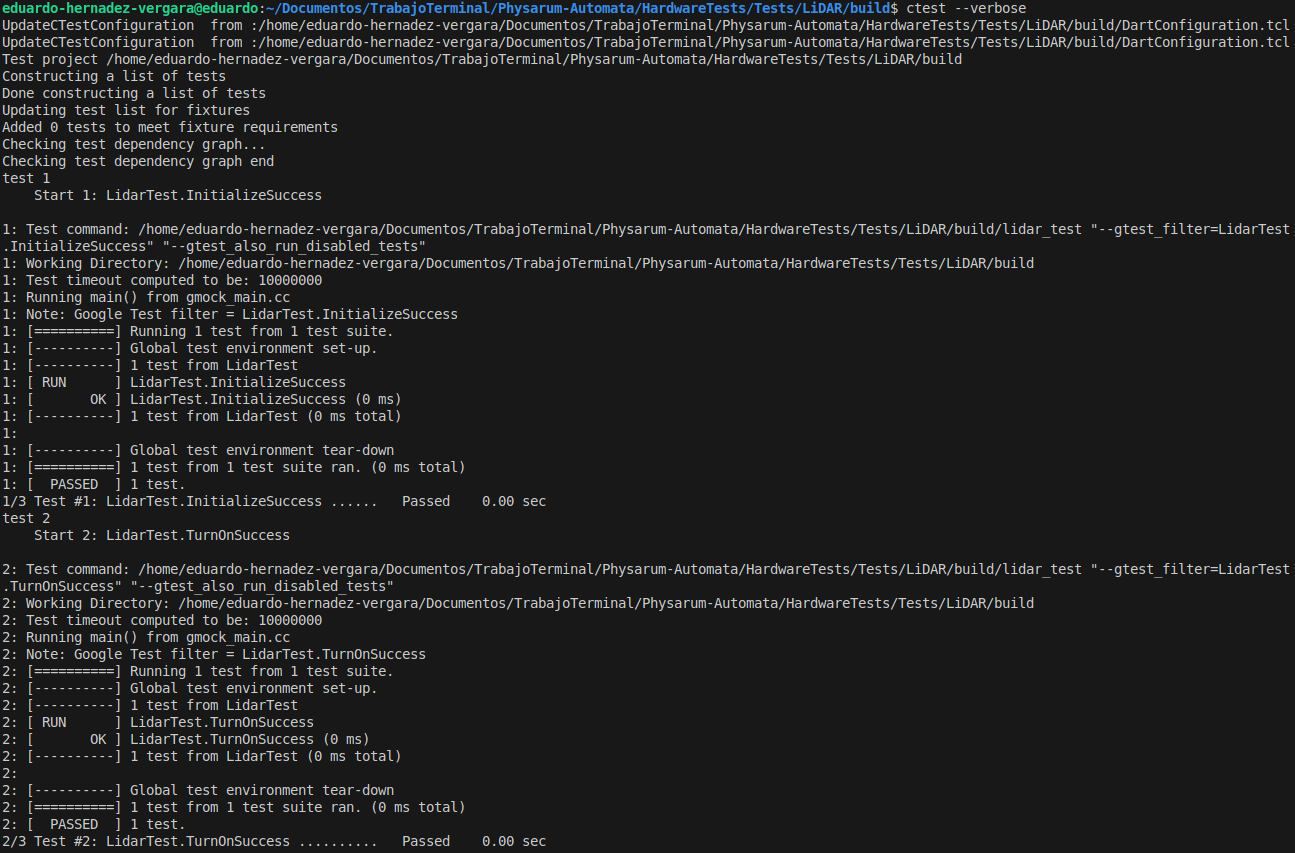
\includegraphics[width=0.8\textwidth]{./images/Pruebas/robot/PruebaLidar01-1.png}
        \caption{Pruebas unitarias del LiDAR 01}
        \label{fig:LidarTest1}
    \end{figure}
    \begin{figure}[htbp]
        \centering
        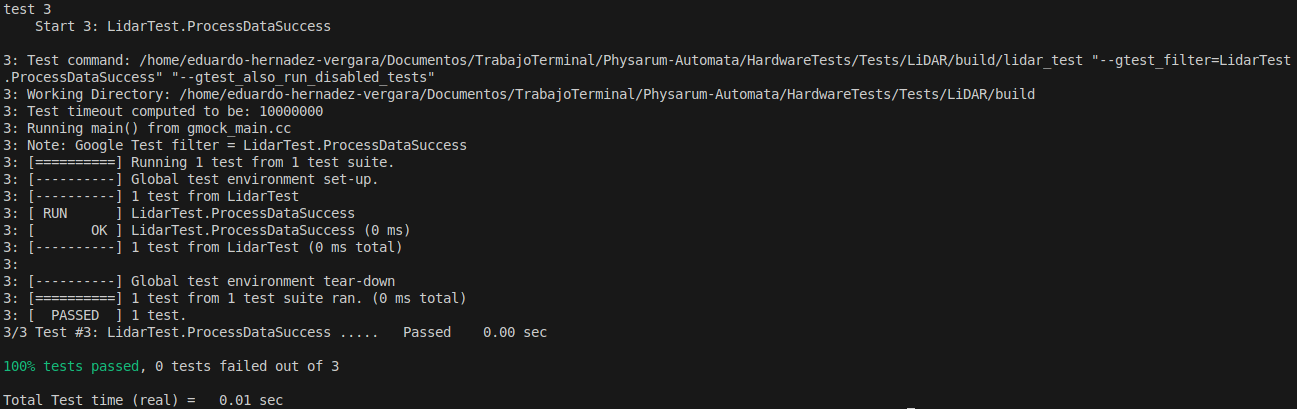
\includegraphics[width=0.8\textwidth]{./images/Pruebas/robot/PruebaLidar01-2.png}
        \caption{Pruebas unitarias del LiDAR 02}
        \label{fig:LidarTest2}
    \end{figure}
    \begin{figure}[htbp]
        \centering
        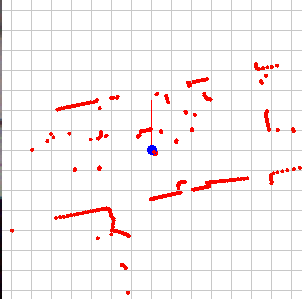
\includegraphics[width=0.8\textwidth]{./images/Pruebas/robot/LidarSFML01.png}
        \caption{Minimapa dibujado con SFML con la informaci\'on del LiDAR}
        \label{fig:LidarTest2}
    \end{figure}
    